\section{Jonosfärskikten}
\textbf{
HAREC a.\ref{HAREC.a.7.3}\label{myHAREC.a.7.3}
}
\index{jonosfär}
\index{jonosfärsskikt}

\emph{Jonosfären} har fått namnet från begreppet jon, som är en fri elektron
eller annan laddad partikel.
Jonisering- elektrisk uppladdning av jordatmosfären sker mellan ca 40--400~km
över jordytan.
Där är lufttrycket tillräckligt lågt för att joner ska kunna röra sig fritt
under avsevärd tid utan att kollidera och återförena sig till neutrala atomer.

När en radiovåg passerar genom ett joniserat skikt i atmosfären,
kan vågen ändra riktning, vilket kallas för refraktion.
För att refraktion ska uppstå måste i första hand två villkor uppfyllas, det
första är tillräckligt tät jonisering och det andra är tillräckligt lång
våglängd.
Under ''gynnsamma'' omständigheter kan vågorna till och med böjas av ner mot
jorden, vilket är den viktigaste förutsättningen för långväga
radioförbindelser på kortvåg.

Joniseringen av atmosfären är emellertid oregelbunden och varierar
bl.a. med höjden över jordytan, solinstrålning, tidpunkt m.m.
Ett antal joniserade skikt kan definieras.
Se bild \ref{fig:bildII7-7}.

\subsection{D-skiktet}
\index{jonosfärsskikt!D-skiktet}

\emph{D-skiktet} förekommer under den ljusa delen av dygnet på en höjd av ca
50--90~km.
På 70--90~km höjd orsakas joniseringen huvudsakligen av röntgenstrålar från
solen, medan den kosmiska strålningen har störst påverkan på 50--70~km höjd.
D-skiktet dämpar de infallande radiovågorna, med största verkan i
kortvågsområdets lågfrekventa del och under de ljusaste timmarna under sommaren.
D-skiktet har dålig reflexionsförmåga och verkar hindrande på
långdistansförbindelser.

\subsection{Mögel-Dellinger-effekten}
\index{Mögler-Dellinger-effekten}
\index{jonosfärsskikt!black out}

Strålning från gasutbrott på solytan kan jonisera D-skiktet så
kraftigt, att alla radiovågor med frekvenser över ca 1~MHz dämpas helt,
detta kallas för \emph{Mögel-Dellinger-effekten}.
Radiotrafik som baseras på vågutbredning via jonosfären är då
omöjlig att genomföra under en tidsrymd av ett antal minuter upp till
flera timmar -- det blir ''black out''.

\subsection{E-skiktet}
\index{jonosfärsskikt!E-skiktet}

\emph{E-skiktet} (Kenelly-Heaviside-skiktet) är det lägsta reflekterande
jonosfärskiktet.
Det förekommer på en höjd av ca 90--140~km och är mest koncentrerat på
ca 110~km höjd.
E-skiktet alstras av att ultraviolett strålning joniserar syreatomer.
Skiktet reflekterar vågor bäst i kortvågsområdets lågfrekventa del och är
kraftigast under den ljusa delen av dygnet.
På grund av D-skiktets dämpande verkan under de ljusaste timmarna är E-skiktet
mest användbart under grynings- och skymningstimmarna.

Ett säsongmaximum i reflexionsförmågan inträffar under sommaren.
Förbindelseavstånd på upp till 2000~km är möjliga.

\subsection{Sporadiska E-skiktet}
\index{jonosfärsskikt!sporadiska E-skiktet}
\index{sporadiska E-skiktet}

Den starkare solinstrålningen under sommaren orsakar en kraftigare
jonisering i den lägre jonosfären än under vintern.
Inom E-skiktet bildas då sporadiska tunna molnlika partier med mycket hög
joniseringsgrad och stor reflexionsförmåga, det s.k. \emph{sporadiska E-skiktet}
(\(E_s\)).
Vågutbredningen via \(E_s\) är mycket olika på olika latituder och är bäst
omkring 40:e latituden.
Mycket goda långväga förbindelser kan uppnås.

\begin{figure}
  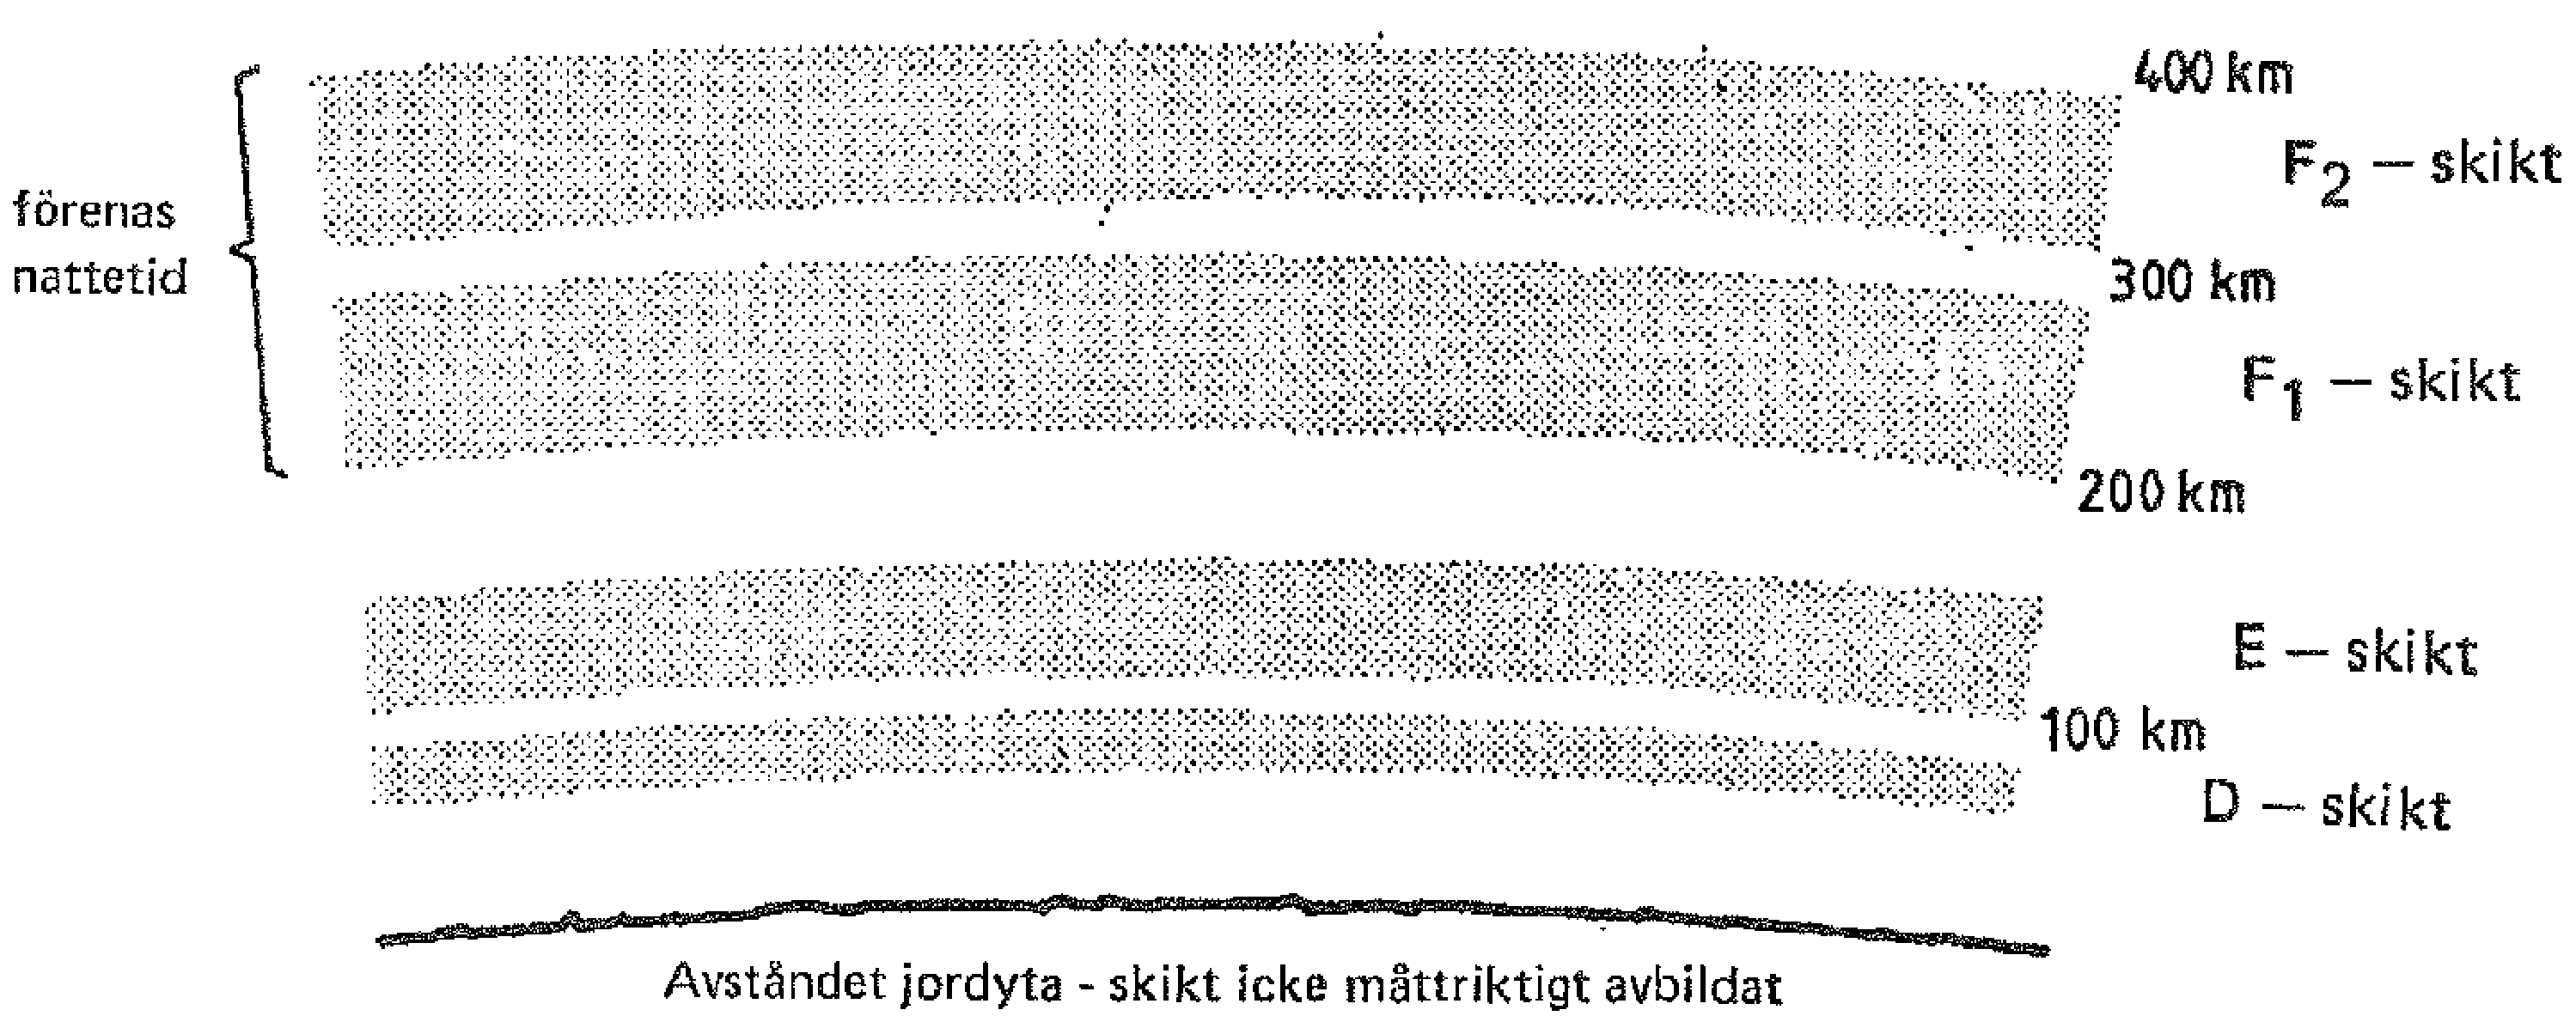
\includegraphics[width=\textwidth]{images/cropped_pdfs/bild_2_7-07.pdf}
  \caption{Jonosfärskikten}
  \label{fig:bildII7-7}
\end{figure}

\subsection{F-skiktet}
\index{jonosfärsskikt!F-skiktet}
\index{F-skiktet}
\index{F1@\(F_1\)}
\index{F2@\(F_2\)}

\emph{F-skiktet} är det högst liggande jonosfärsskiktet.
Det förekommer såväl dag- som nattetid på en höjd av 140--500~km.
Den nedre del av skiktet, 140--200~km, uppvisar andra variationer än den övre
delen.
F-skiktet beskrivs därför som två skikt, \(\mathrm{F_1}\) upp till ca 200~km
höjd och \(\mathrm{F_2}\) över denna höjd.

Liksom E-skiktet, påverkas \(\mathrm{F_1}\)-skiktet kraftigt av
instrålningen från solen.
Det når sin högsta joniseringsgrad ungefär en timme efter högsta lokala
solståndet och förekommer endast under sommaren.
Under natten förenar sig \(\mathrm{F_1}\)- och \(\mathrm{F_2}\)-skikten till
ett enda F-skikt.

\(\mathrm{F_2}\)-skiktet är det skikt som varierar mest i tiden och rummet.
Den högsta joniseringsgraden inträffar vanligen sent efter högsta lokala
solståndet, ibland under aftontimmarna.
Skiktets maximala jonisering är på 250--350~km höjd på mellanlatituder och på
350--500~km höjd vid ekvatorn.
På mellanlatituder ligger den största elektrontätheten i skiktet högre under
natten än under dagen.
Vid ekvatorn är förhållandet omvänt.

Reflexioner i \(\mathrm{F_2}\)-skiktet möjliggör att stora
avstånd kan överbryggas (1 hopp = 3000--4000~km).

\begin{figure}
  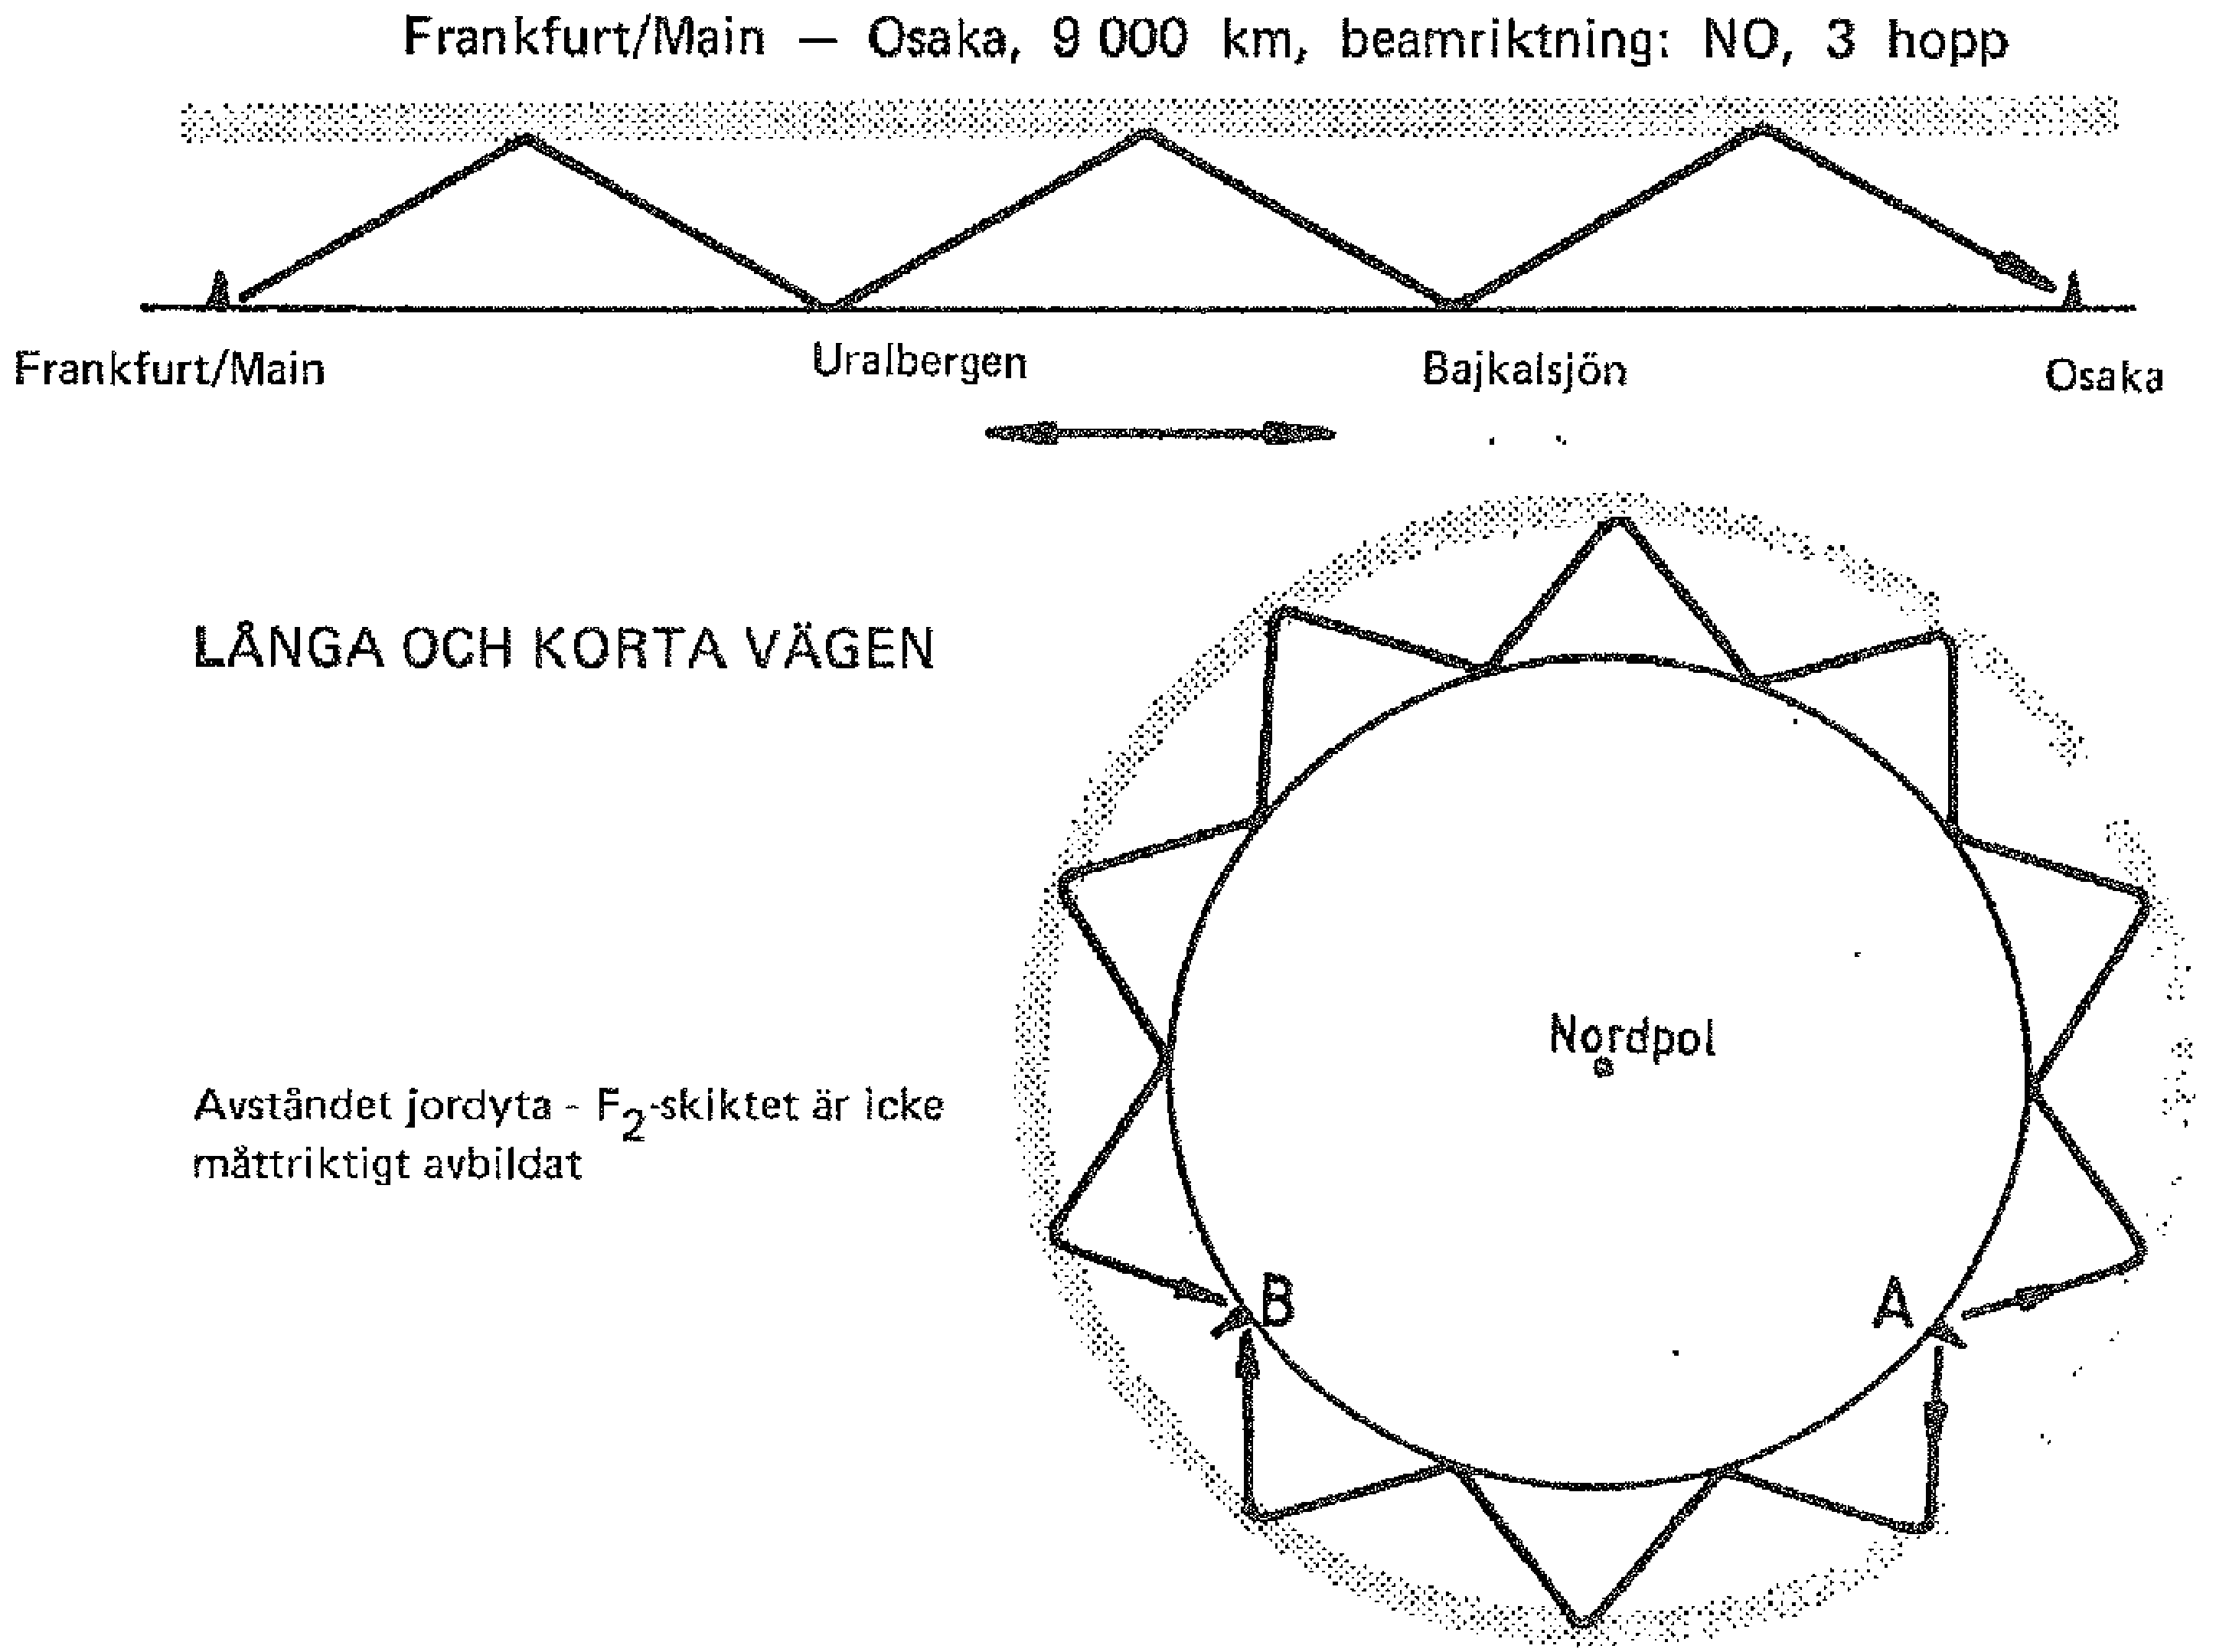
\includegraphics[width=\textwidth]{images/cropped_pdfs/bild_2_7-08.pdf}
  \caption{Jonosfärsutbredning.}
  \label{fig:bildII7-8}
\end{figure}

\subsection{Höjd till reflekterande skikt}
\index{jonosfärsskikt!höjd till skikt}

När en radiovåg, som riktas rakt uppåt, träffar jonosfären kan den antingen
\begin{itemize}
  \item absorberas -- sugas upp
  \item reflekteras
  \item tränga igenom.
\end{itemize}

Vilket som inträffar beror på den använda frekvensen.
Ju högre frekvensen är på den uppåtriktade radiovågen, desto högre upp i ett
atmosfärskikt kommer avböjningen tillbaka att inträffa.
Höjden till skiktet beräknas ur radiovågens utbredningshastighet och
utbredningstid fram och åter mellan skiktet och jordytan.

\subsection{Kritisk frekvens}
\textbf{
HAREC a.\ref{HAREC.a.7.4}\label{myHAREC.a.7.4}
}
\index{kritisk frekvens}

Vid en viss övre frekvens upphör reflexionen i atmosfärskiktet och
vågen går ut i rymden i stället för ner till jordytan.
Denna frekvens kallas den \emph{kritiska frekvensen}, som varierar med
joniseringsgraden i atmosfären.
Den kritiska frekvensen är högst vid högt solfläckstal, såväl i E- som i
F-skikten, eftersom joniseringsgraden då är störst.
Den kritiska frekvensen för E-skiktet varierar mellan ca 1--4~MHz beroende på
tidpunkt i solfläckscykeln och tid på dagen.
Den kritiska frekvensen för F-skiktet varierar med tid på dagen, årstid och
skede i solfläckscykeln.
Den kan variera från 2--3~MHz natten under ett solfläcksminimum till 12--13~MHz
på dagen under ett solfläcksmaximum.

\subsection{Kritisk vinkel}
\index{kritisk vinkel}

Rymdvågen måste träffa ett joniserat atmosfärskikt med en tillräckligt
flack vinkel för att reflekteras, den s.k. kritiska vinkeln.
Denna vinkel är frekvensberoende.
Allt eftersom den utsända frekvensen ökas ytterligare över den kritiska
frekvensen, måste vågen träffa atmosfärskiktet i en allt flackare vinkel för att
vågen ska reflekteras mot jordytan.
Genom att sända ut vågen i mycket flack vinkel
mot \(\mathrm{F_2}\)-skiktet kan långa distanser överbryggas vid
frekvenser som är upp till 3,5 gånger den kritiska frekvensen.

Så snart den kritiska frekvensen är högre än frekvensområdet för ett
amatörband är det alltså möjligt att kommunicera över rymdvåg på detta band.
Det kan ske över alla avstånd, allt ifrån skipavståndet till det
som avgörs av utbredningsförlusterna.

\subsection{Högsta användbara frekvens (MUF)}
\textbf{
HAREC a.\ref{HAREC.a.7.6}\label{myHAREC.a.7.6}
}
\index{högsta användbara frekvens}
\index{MUF}
\index{Maximum Usable Frequency (MUF)}

Radiovågorna vandrar från sändaren till en avlägsen mottagare genom
att reflekteras en eller flera gånger i jonosfären och på jordytan. 
För att detta ska ske kan frekvensen inte vara högre än den
\emph{högsta användbara frekvensen} (eng. \emph{Maximum Usable Frequency (MUF)})
för en viss överföringssträcka.

MUF är högst mitt på dagen eller tidig eftermiddag.
Allra högst är MUF under perioder av högt solfläckstal och kan då komma
upp till över 30~MHz.
Under tidiga morgontimmar sjunker MUF ofta under 5~MHz.

De jonosfäriska förlusterna är lägst nära MUF och ökar snabbt under
dagtid för lägre frekvenser.

Aktuella MUF-data publiceras periodiskt i olika media, men kan också
överslagsberäknas med hjälp av speciella datorprogram.

\subsection{Optimal trafikfrekvens (FOT)}
\index{optimal trafikfrekvens}
\index{FOT}

I praktiken är det av intresse att veta det frekvensområde där
kommunikation bäst kan genomföras.

Rekommenderad övre frekvensgräns för en tillförlitlig radioförbindelse
kallas \emph{optimal traffic frequency (FOT)} och väljs något under
MUF som marginal för oregelbundenheter och turbulens i jonosfären,
liksom för korttidsavvikelser från det förutsagda månatliga
medianvärdet för MUF.
FOT är vanligen ungefär 15~\% lägre än MUF.

\subsection{Lägsta användbara frekvens (LUF)}
\index{lägsta användbara frekvens}
\index{LUF}
\index{Lowest Usable Frequency (LUF)}

Ju lägre sändningsfrekvens som väljs, desto mer dämpas vågorna i
jonosfären, intill den frekvens då de inte kan uppfattas.
Den \emph{lägsta användbara frekvensen}
(eng. \emph{Lowest Usable Frequency (LUF)}) är den
frekvens som ger tillfredsställande kommunikation för en viss
utbredningsväg och vid en viss tidpunkt.

Vid frekvenser under LUF är mottagning inte möjlig eftersom brusnivån
då är för hög.
Ju mer frekvensen höjs över LUF, desto bättre blir signal-brus-förhållandet.

Till skillnad från MUF, som endast påverkas av de jonosfäriska
förhållandena, kan LUF till en del påverkas genom utsänd effekt och bandbredd.
Generellt kan LUF sänkas ca 2~MHz för varje 10~dB ökning av E.R.P.

\subsection{Vågutbredningsförutsägelser}
\index{vågutbredningsförutsägelser}
\index{vågutbrednings!förutsägelser}
\index{vågutbredning!propagation forecasts}
\index{ursigram}
\index{URSI}
\index{Union Radio-Scientifique Internationale (URSI)}

Det görs regelmässiga förutsägelser av de jonosfäriska förhållandena.
Fortlöpande fysiska observationer, statistisk och matematisk bearbetning ligger
till grund för förutsägelserna, vilka bl.a. utnyttjas för att planera
radiotrafiken.
Vågutbredningsförutsägelser (propagation forecasts) som ger upplysningar om de
lämpligaste frekvenserna och tiderna för olika förbindelsesträckor görs av både
civila och militära institutioner. 
Tidigare meddelades sådana förutsägelser i offentliga publikationer samt i 
amatörradions tidskrifter och bulletiner.

Idag finns i stort sett alla vågutbredningsförutsägelser, data över
solaktiviteten och information om det geomagnetiska fältet fritt tillgängligt på
Internet.

En sökning på nätet efter \emph{propagation forecast ham radio} ger träffar på
många webbplatser.
SSA:s webbplats har i högermarginalen information om \emph{solar terrestrial data}
och \emph{calculated conditions}.

Förr var vågutbredningsförutsägelser endast tillgängliga som \emph{Ursigram} som
skickades per telex eller brev från \emph{Union Radio-Scientifique
Internationale (URSI)}.

Ursigrammen kunde erhållas genom ett dyrt årsabonnemang och de innehöll aktuella
mätvärden såsom solfläckstal \(R\), 10~cm solflux \(F\), magnetiskt index \(K\)
och gränsdämpningsvärden.
De kunde även innehålla anvisningar om särskilda händelser (flares,
magnetstormar, polarkalott absorption, Mögel-Dellinger-effekter och liknande).

Bild \ref{fig:bildII7-9} visar en radioprognos för juni 1997 ur SSA:s
medlemstidning QTC.
Tabellen i bilden visar sannolikheten i procent för att få förbindelse på de
olika kortvågsbanden från Sverige till andra länder och världsdelar.

Trots sin höga ålder ger tabellen en bild över hur möjligheten att få en
förbindelse på kortvåg varierar med frekvens och tid på dygnet.
Observera även det låga solfläckstalet SSN (Sun Spot Number).

\begin{figure}
  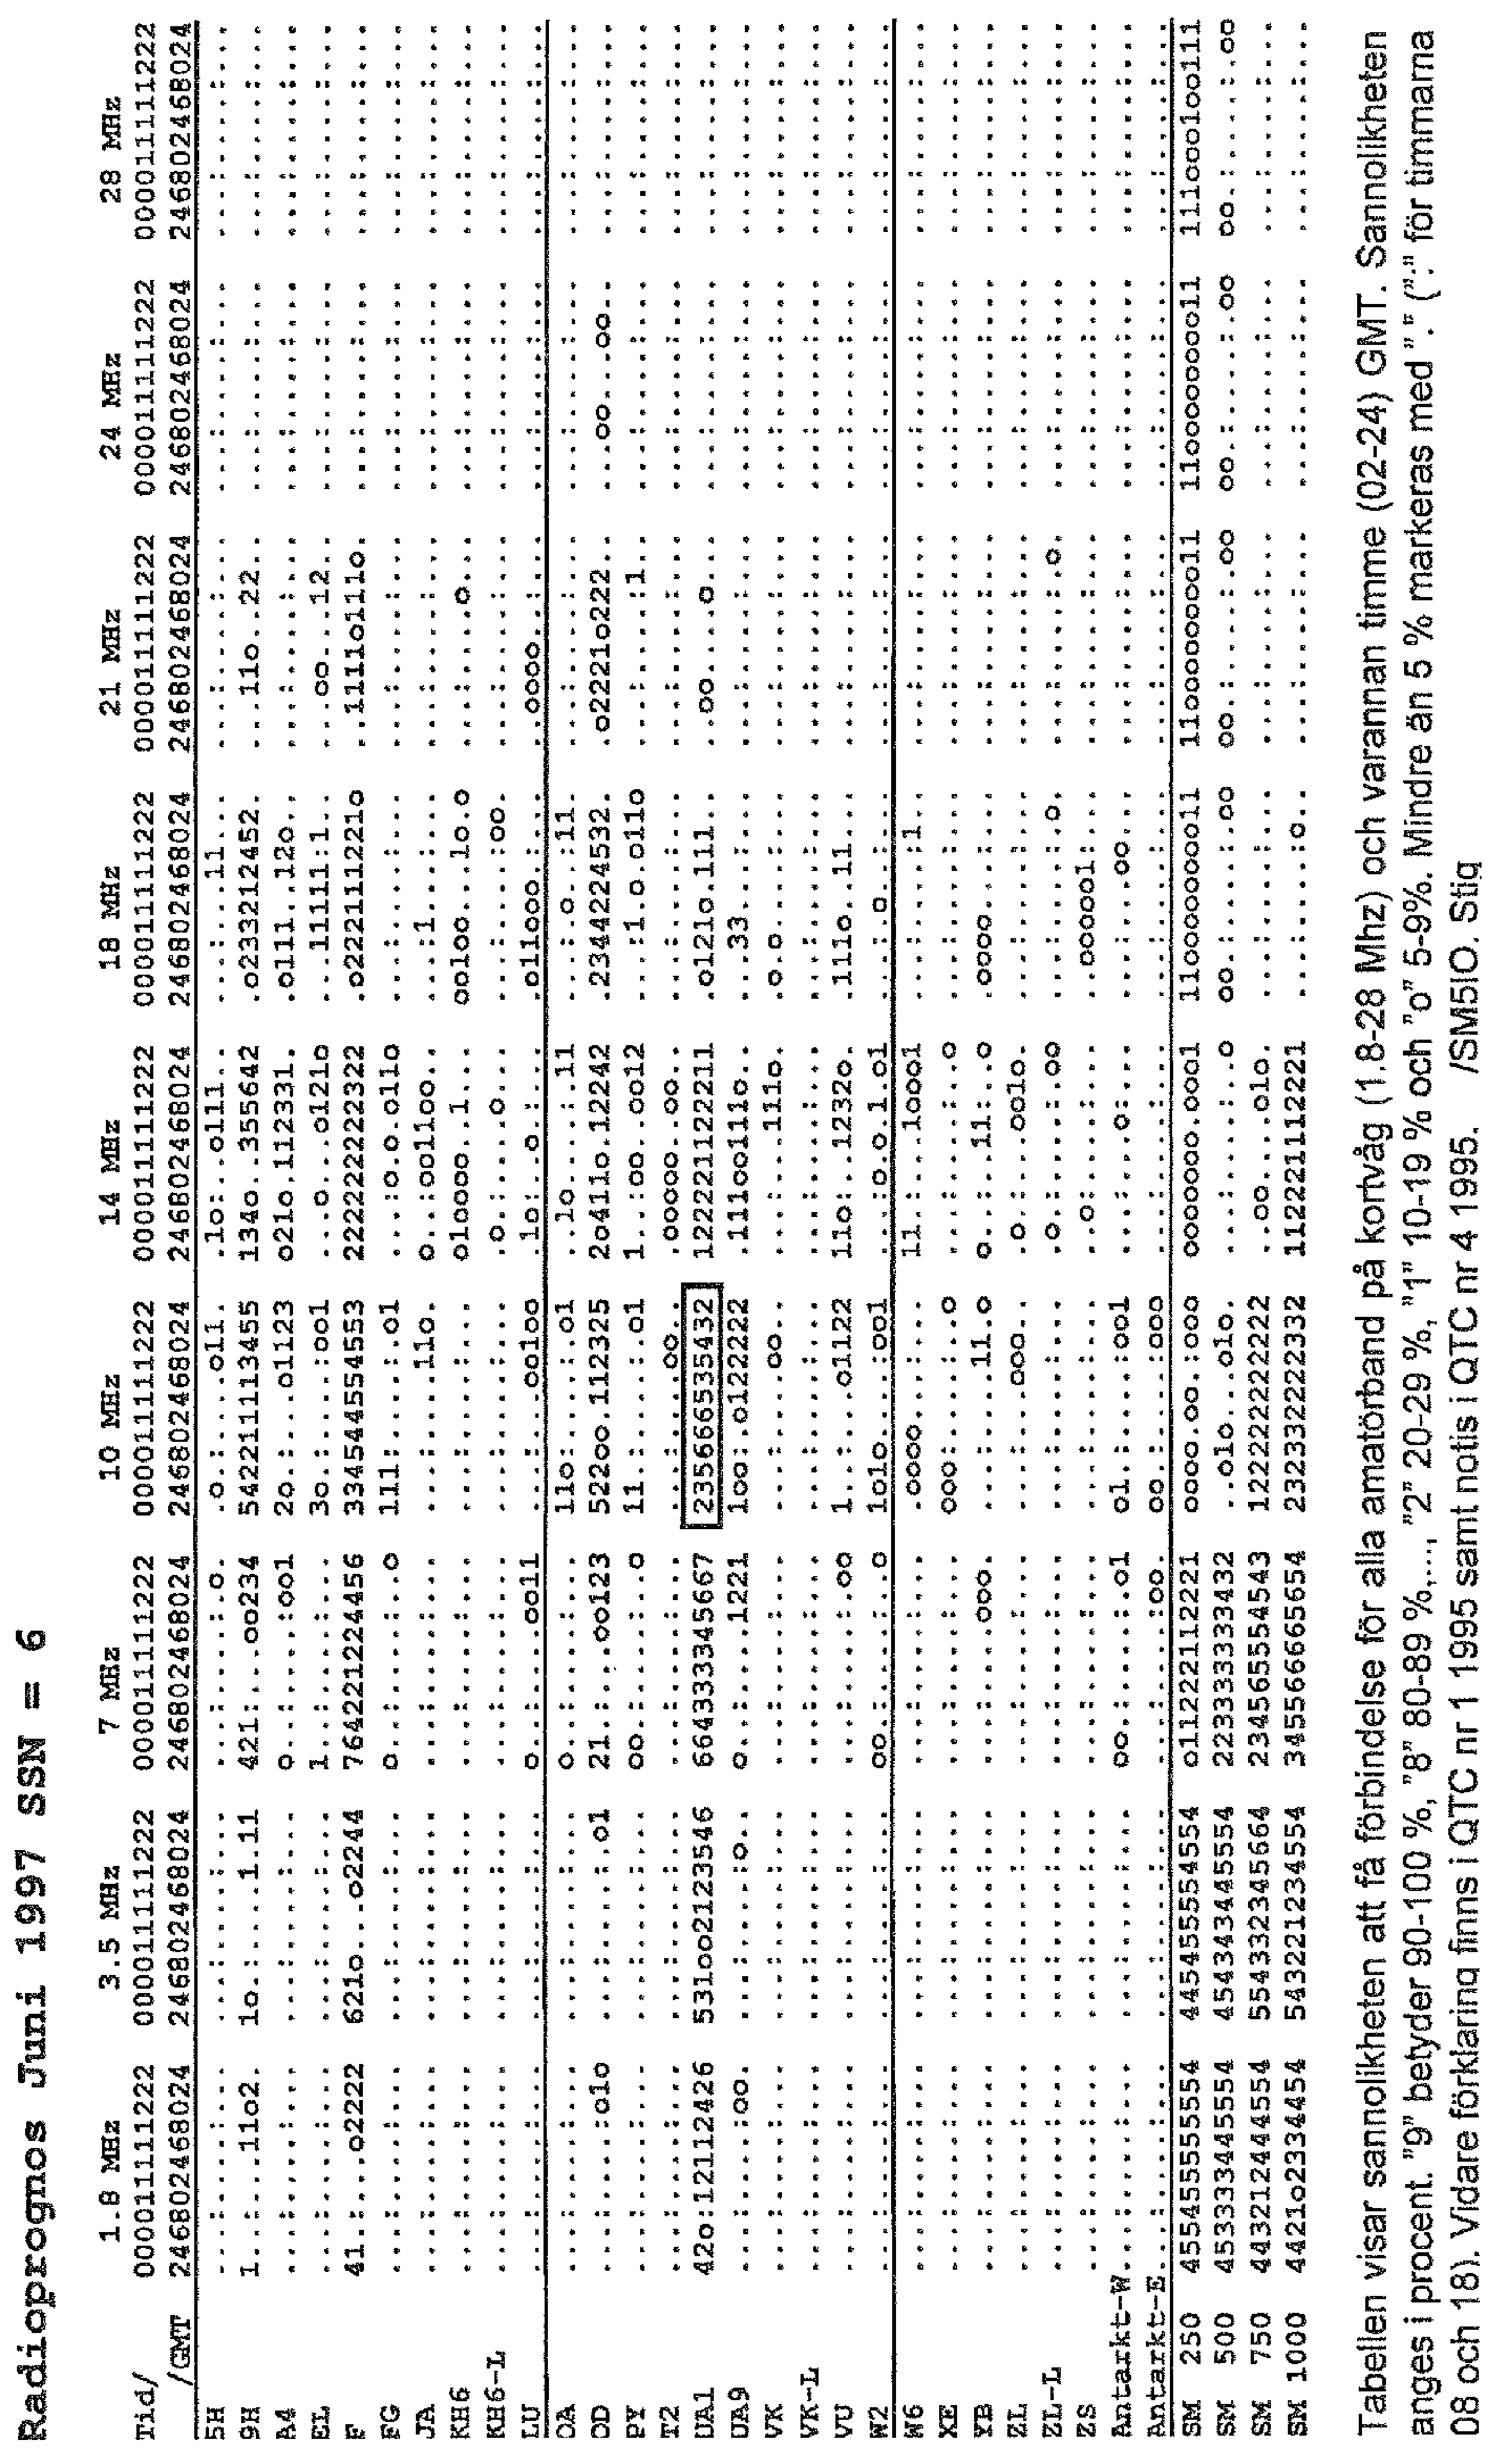
\includegraphics[width=\textwidth]{images/cropped_pdfs/bild_2_7-09.pdf}
  \caption{Radioprognos för amatörradiobanden på kortvåg}
  \label{fig:bildII7-9}
\end{figure}
